\section{Combustion Instabilities}

\subsection{Thermoacoustic Instability}


Combustion for engineering applications typically happens in systems of chambers, connected by long ducts. Although the chemical and hydrodynamic scales remain relatively short, and are localised to specific areas, e.g. the combustion chamber, acoustics travel throughout the system without significant damping due to the acoustically reflective materials used. Hence, the dominant acoustic eigenmodes of a system are therefore free to interact with the flame as they please. The resulting \emph{thermoacoustic} (TA) instabilities are classed as a form of chamber instability due to the reliance of the flame's spontaneous acoustics on specific geometries. The effect of thermoacoustics was first noticed in \cite{mallard1883RecherchesExperimentalesTheoriques}, where it was observed that flames can produce their own acoustic oscillations. Following this, \cite{rayleigh1896TheorySound} introduced a theoretical condition for a \emph{primary} TA instability, so called the \emph{Rayleigh criterion}, where fluctuations in pressure and heat release from the flame are amplified whenever they are in phase. To explain this in more detail, periodic changes to pressure are coupled to changes in acoustic velocity. This has a convective effect on the shape of the curved, hydrodynamically unstable \cite{darrieus1945PropagationFrontFlamme,landau1944TheorySlowCombustion,matalon2018DarrieusLandauInstability} flames, resulting in an oscillation of the total heat release. This causes further oscillations to the radiated acoustic pressure from the flame, which closes this feedback mechanism. The primary TA instability can, hence, only occur when the oscillating pressure around the flames results in heat release oscillations which add to the acoustic pressure amplitude. Mathematically, instability is triggered whenever:
\begin{equation}
\rm{RI} \equiv \oint p' Q' \dd{t} > 0
\end{equation}
where $\rm{RI}$ is the \emph{Rayleigh Index}, $p'$ and $Q'$ represent fluctuations in the pressure and total heat release, respectively. The closed integral sign represents the integral over a single of the above mentioned periods. This statement translates to the statement that $p'$ and $Q'$ must be in phase with one another for instability to occur. This phase is controlled by the acoustics of the combustion chamber itself so small changes to combustor system's geometry can result in large qualitative changes to stability. When they are in phase, the feedback loop takes the form of a clockwise p-V cycle \cite{polifke2004CombustionInstabilities}, equivalent to an Otto cycle. This means the mechanism can generate mechanical work which, when confined to an engine, can take the form of a damaging force on engine parts, such as the damage observed in \cite{lieuwen2006CombustionInstabilitiesGas}.

\begin{figure}[t]
\centering
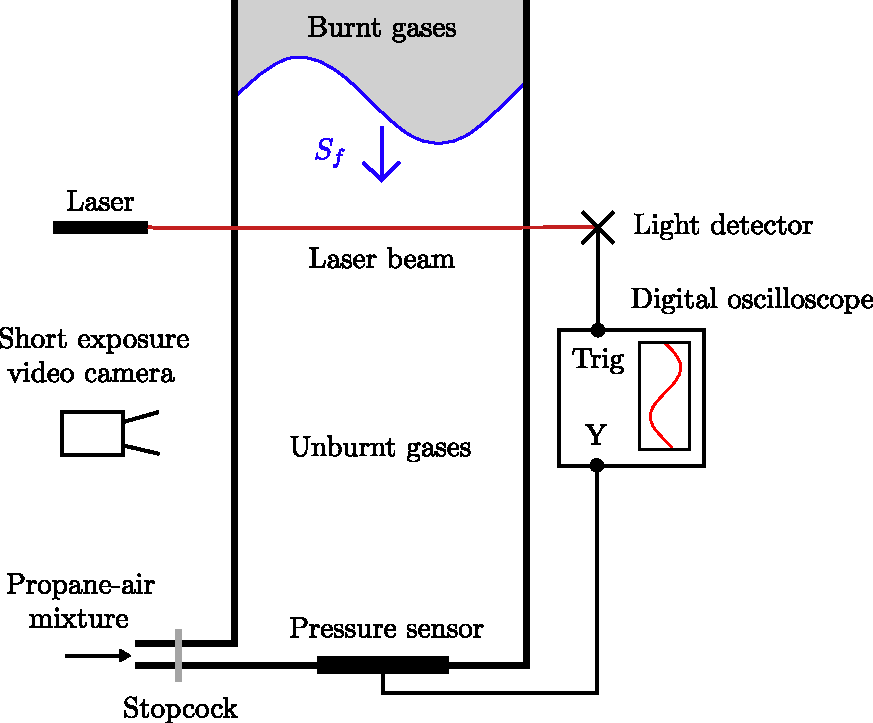
\includegraphics[scale=0.6]{assets/imgs/Searby-92.pdf}
\caption{Illustration of the experimental apparatus of \cite{searby1992AcousticInstabilityPremixed}.}
\label{fig:searby-experiment}
\end{figure}

A crucial experiment into thermoacoustics was performed by Searby in 1992 \cite{searby1992AcousticInstabilityPremixed}, which studied the correlation between the acoustics detected in a long, thin tube and the speed and shape of the laminar premixed flame within, depicted in \fig{fig:searby-experiment}. Propane-air mixtures were lit at the top end of the tube and propagate down, with any acoustic disturbance detected by a pressure sensor at the bottom. Additionally, a small laser beam was place near the top of the tube to detect the flame as thermal gradients deflect the light. This triggers a digital oscilloscope to record pressure disturbances from the pressure sensor. A short exposure video camera was used to image the flame surface and observe its structure as it propagates. Since propane (C$_3$H$_8$) is a relatively heavy fuel with a species diffusion rate lower than methane's, the lean and stoichiometric mixtures used have Lewis numbers which are never below the critical Lewis number, $\Le_\rm{crit}$, required for \emph{thermodiffusive instabilities} \cite{zeldovich1944TheoryCombustionDetonation,barenblatt1962DiffusionalThermalStabilIty,sivashinsky1977DiffusionalThermalTheoryCellular} to have an effect. Note that the downward propagating flames will have been somewhat stabilised by the \emph{Rayleigh-Taylor} (RT) instability. The primary instability is observed alongside a secondary, which is associated with a different feedback mechanism, acoustic envelopes and flame dynamics.

\begin{figure}[t]
\centering
\begin{subfigure}{0.49\textwidth}
\centering
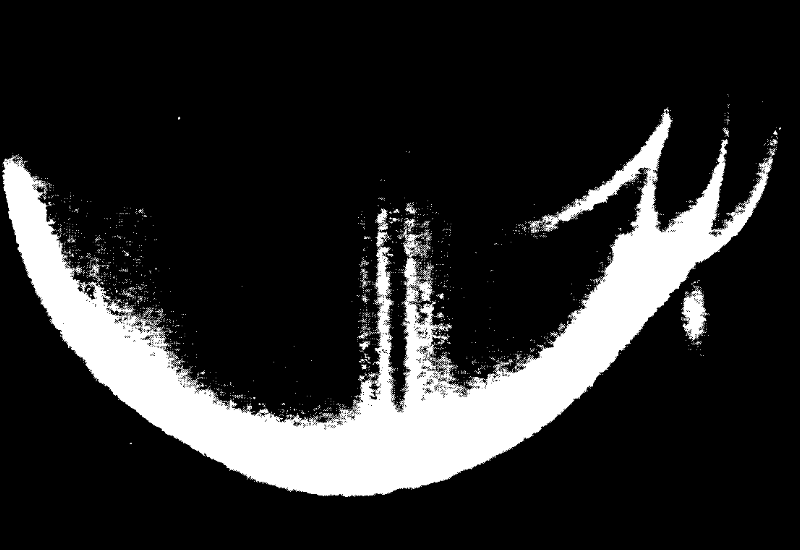
\includegraphics[height=5cm]{assets/imgs/Searby-92-flame_a.png}
\caption{}
\label{fig:Searby-92_flames_a}
\end{subfigure}
\hfill
\begin{subfigure}{0.49\textwidth}
\centering
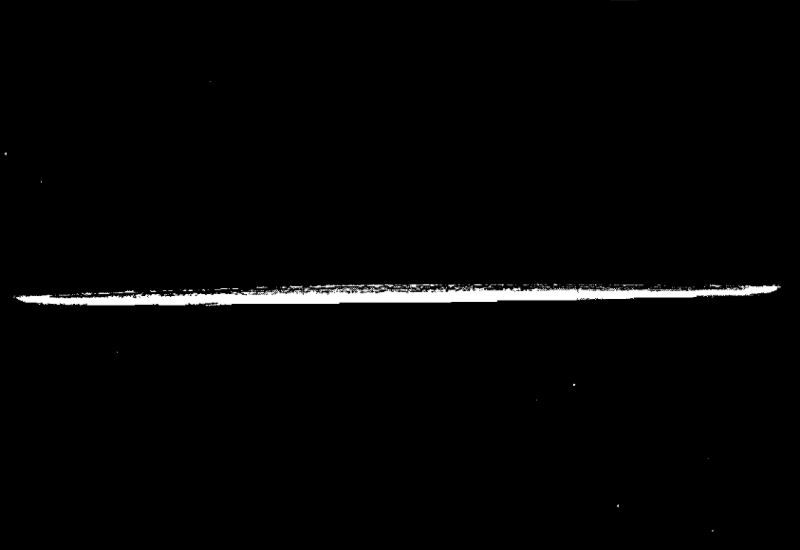
\includegraphics[height=5cm]{assets/imgs/Searby-92-flame_b.png}
\caption{}
\label{fig:Searby-92_flames_b}
\end{subfigure}

\vspace*{3mm}

\begin{subfigure}{0.49\textwidth}
\centering
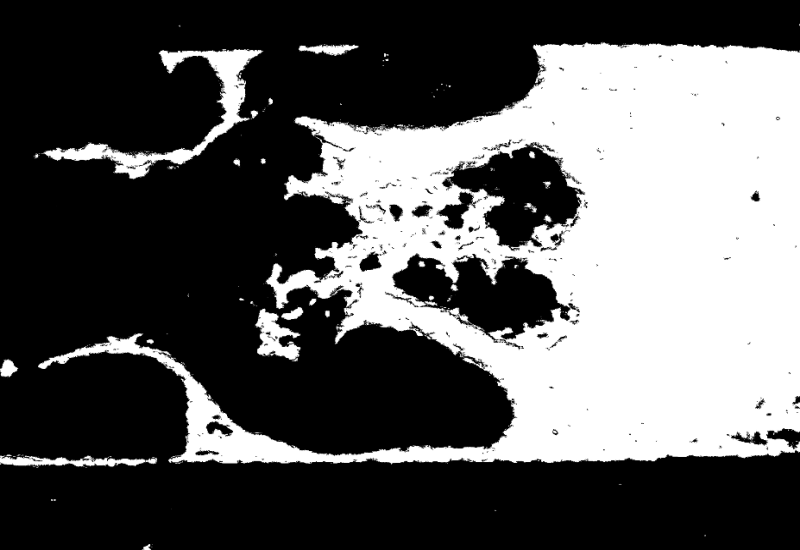
\includegraphics[height=5cm]{assets/imgs/Searby-92-flame_c.png}
\caption{}
\label{fig:Searby-92_flames_c}
\end{subfigure}
\hfill
\begin{subfigure}{0.49\textwidth}
\centering
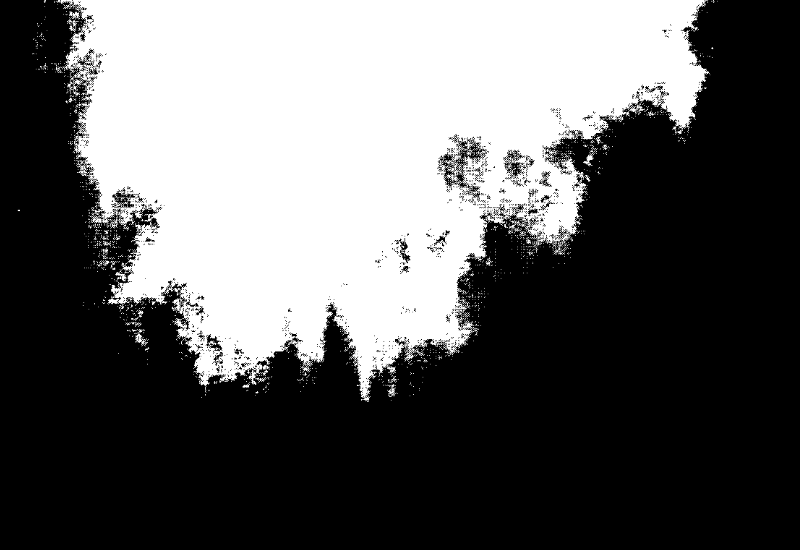
\includegraphics[height=5cm]{assets/imgs/Searby-92-flame_d.png}
\caption{}
\label{fig:Searby-92_flames_d}
\end{subfigure}
\caption{Photos, courtesy of \cite{searby1992AcousticInstabilityPremixed}, of flames at different stages of thermoacoustic response. (a) shows the characteristic curved shape of a hydrodynamically unstable flame before any acoustics are significantly effecting the flame shape. (b) is a flame flame under the effect of the primary thermoacoustic instability. (c) shows a cross-sectional slice of a flame rotated by $90\degree$ under the secondary instability. (d) shows a flame after the breakdown of cellular structures, which leads to a self-turbulent flame.}
\label{fig:Searby-92_flames}
\end{figure}

Initially, the flame curves as a result of the hydrodynamic instability, as photographed in \fig{fig:Searby-92_flames_a}. After some time, the acoustic amplitude increases due to primary instability. As the acoustic amplitude increases the flame flattens, seen in \fig{fig:Searby-92_flames_b}, resulting in a decrease in flame speed due to the decreased fuel consumption rate. In some of the flames tested, only the primary instability is observed, but in some others it progresses beyond this to the secondary instability -- often before the fully flattened flame is observed. At the immediate onset of the secondary instability, if it occurs, a cellular structure of a given wavenumber appears and corresponds to a rapid increase in the acoustic amplitude. This onset is much more rapid than for the primary instability, and eventually the cellular structure transitions into a symmetric flame structure similar to \fig{fig:Searby-92_flames_c}. Provided the flame has not yet reached the end of the tube it may also devolve into a self-turbulent flame similar to that shown in \fig{fig:Searby-92_flames_d}. The flame structures resulting from the secondary instability have significantly higher velocities as a result of their massively increased flame surface area and are viewed as a violent instability. The self-turbulent regime marks a significant decline to the acoustic amplitude as there is no regular release of pressure fluctuations from the flame.

% Flat flame under primary can be seen as a limit cycle

Following this, thermoacoustic oscillations have been observed in a variety of experimentation.

Methane-air combustion in a cylindrical tube was investigated experimentally in \cite{fichera2001ExperimentalAnalysisThermoacoustic} with data recorded from an optical sensor to detect changes to heat release, a pressure transducer for internal pressure recordings and a microphone for external pressure recordings. Thermoacoustic oscillations were observed and a non-linear analysis into the dynamical behaviour of the flame recordings demonstrate a chaotic nature to these thermoacoustics. The global stability of the flame, which is guaranteed by diffusive effects, is corroborated via calculation of the set of Lyapunov exponents.

SOME NEW CHANGE



% Following this, thermoacoustic oscillations have been observed in a variety of experimentation:
% delfin2024ThermoacousticParametricInstability
% - High resolution and speed images of flames under thermoacoustic instability in open-ended tubes as well as clear images of flame structure under parametric instability

% ebieto2017DynamicsPremixedFlames (THESIS)
% - high speed imaging of a variety of thermoacoustic flames

% tachibana2015ExperimentalNumericalInvestigation
% - spray combustion in a liquid-fuel aero-engine
% - experiment vs LES

% For high quality examples of thermoacoustic oscillations in motion, one can refer to
% delfin2024VideoTransientParametric
% martinez-ruiz2018VideoPremixedflameOscillations







The secondary instability mechanism is seen by Searby \cite{searby1992AcousticInstabilityPremixed} as a \emph{parametric instability}. Physically, this is where one mode of a system at some frequency and another mode at twice the first frequency excite each other to form a positive feedback loop. In our thermoacoustic instabilities, this first mode is the flame structure which oscillates at half the frequency of the pressure fluctuations.

Substitutions performed in \cite{searby1986WeaklyTurbulentWrinkled} show that a downward propagating flame in two-dimensions under the influence of gravity may have its flame surface written as a damped harmonic oscillator:

Incorporating the force acoustics have on the flame position gives us an equation which can again be reposed as the Mathieu equation \cite{searby1991ParametricAcousticInstability}:


% EXPLAIN WHAT S_L AND L_TH ARE
\begin{figure}[t]
\centering
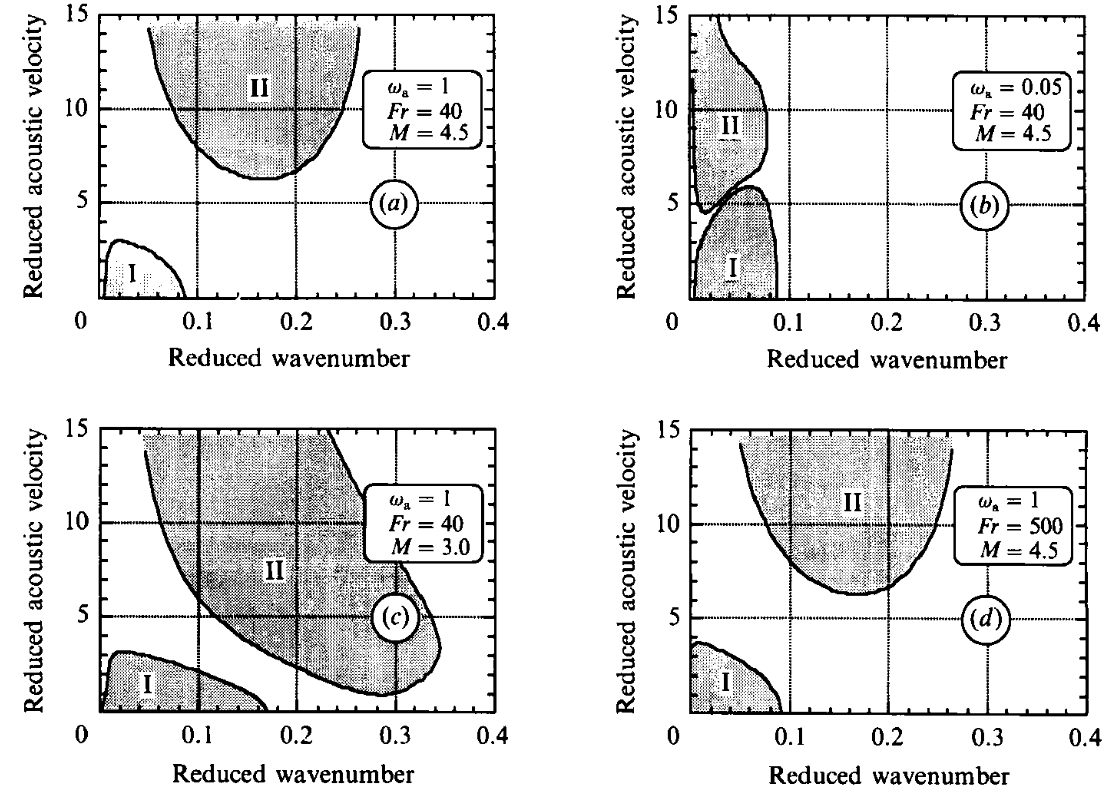
\includegraphics[height=11cm]{assets/graphs/thermoacoustic-stability.png}
\caption{Stability diagrams, courtesy of \cite{searby1991ParametricAcousticInstability}, for four different values of $ω_a$, $\Fr$ and $\Mk$. The regions I and II are regions of instability for the plane flame. Reduced wavenumbers are given as $k l_\rm{th}$ and reduced acoustic velocities are $u_a / S_L$.}
\label{fig:ta-stab}
\end{figure}

Using this formation of the flame front as solutions to the Mathieu equation, Searby and Rochwerger \cite{searby1991ParametricAcousticInstability} calculate regions of flame instability for a planar flame as functions of $k$, $u_a$ (the acoustic velocity, which can be thought of as the intensity or volume of sound), $ω_a$, $\Fr$ and $\Mk$. They then plot these regions in \fig{fig:ta-stab} (note that these plots do not the acoustic instabilities mentioned above, but their effect on the stability of a planar flame). In all the plots, there are two disjoint regions of flame instability. The region I represents the hydrodynamic instability of plane flames and occurs, as we expect, at zero acoustic velocity. This region ends at some finite $u_a$ as the primary acoustic instability eventually overcomes the hydrodynamic one. At non-zero acoustic velocity, region II of flame instability begins and corresponds to the aforementioned parametric instability and is calculated by considering the acoustic velocities for a given wavenumber which will overcome the effects of damping. Interestingly, some of the graphs show acoustic velocities where regions I and II can exist. In these cases, the primary thermoacoustic instability is expected to lead immediately into the secondary instability with not planar flame observed. For those acoustic velocities where neither region is present, the planar flame is stable so we see structures like \fig{fig:Searby-92_flames_b} where the flame has spontaneously flattened before any secondary instability can occur. We also notice that there is a wavenumber in region II which corresponds to the lowest unstable acoustic velocity. This means that once this acoustic velocity is met, only that wavenumber (and wavenumbers close to it) will be present as wrinkles in the flame. Finally, we note that the effect of gravity on these downward propagating flames has stabilised the very low wavenumbers next to region I as the RT effect actually stabilises the plane flame.

An experiment was also performed by \cite{searby1991ParametricAcousticInstability} to demonstrate these results. A similar apparatus to \fig{fig:Searby-92} was used, with significant changes being the usage of a loudspeaker in the bottom of the combustion tube to play sounds of wavelength one-quarter or three-quarters of the wavelength of the tube. A porous plate was placed above the loud speaker to remove any turbulence such that our laminar theories can be applied. Using the loud speaker to excite the flame at known volumes and frequencies (which correspond to controlling $u_a$ and $ω_a$, respectively), they observe both the planar and wrinkled flames described above.





% searby1991ParametricAcousticInstability
% - the nature of this secondary instability is studied by modelling the flame front as the matthieu equation
% - when the forcing term exceeds a certain amplitude, a parametric instability is triggered where the flame shape moves at a subharmonic frequency, half the frequency of the forcing acoustic
% - this is corroborated by images taken in searby1992AcousticInstabilityPremixed
% - Solving these equations(?) gives them numerical predictions the stability regions of the planar flame, where a stable flat flame is observed if and only if a stability band of of sound intensities occurs between the loudest Darrieus-Landau unstable flame and the quietest parametrically unstable flame.
% - The sound intensity corresponding to the quietest parametrically unstable flame may then be plotted for a variety of acoustic frequencies (forced via loudspeaker), which results in a curve predicted by the Markstein number of combustion mixture (provided other constants are known so the curves can be predicted from the theory)




\begin{figure}[t]
\centering
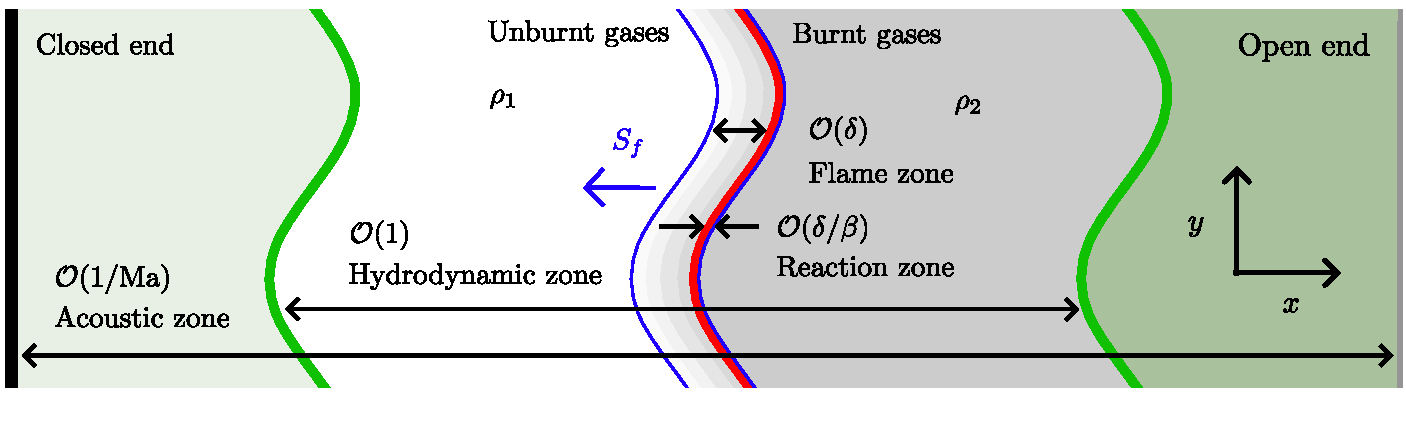
\includegraphics[scale=0.6]{assets/imgs/AW-flame.pdf}
\caption{Diagram showing the model geometry of the multiscale analysis performed by \cite{assier2014LinearWeaklyNonlinear}.}
\label{fig:AW-flame}
\end{figure}

Later on, work by Assier and Wu \cite{assier2014LinearWeaklyNonlinear} studied the stability of a \emph{flame-flow-acoustic} system, where a freely propagating flame in a duct which is periodic to the top and bottom and has one closed and open end to the left and right is considered. \fig{fig:AW-flame} illustrates this geometry, which is reminiscent of the experimental domain shown in \fig{fig:searby-experiment} of \cite{searby1992AcousticInstabilityPremixed}. Results from the hydrodynamic flame theory \cite{matalon1982FlamesGasdynamicDiscontinuities} are used to separate the dynamics within the flame from the outer fluid. This outer region is then separated into the usual $\cl{O}(1)$ hydrodynamic zone and a far-away $\cl{O}(1/\Ma)$ acoustic zone. Further asymptotic analysis is performed in the flame reference frame, which couples these two regions primarily through a time-dependent term in the jump conditions. The same weak non-linearity assumption is made as the MS equation to simplify their form of the flame equation and linear stability analysis is performed about the steady solutions to the MS equation.

They find that, when the acoustic interaction is included these solutions are no longer linearly stable and the maximum growth rate of this instability increases significantly with heat release $q$. They also perform non-linear stability analysis using a solver for the flame position coupled to the dynamical acoustic jump conditions. This is compared to the results of \cite{searby1992AcousticInstabilityPremixed} and they find they are able to qualitatively reproduce the primary instability and the onset of the secondary instability. In the latter case, the unsteady nature of the acoustic coupling to the flame induces an unsteady RT effect as the acoustic acceleration oscillates into and away from the less dense products. This can be viewed as the driving mechanism behind this parametric instability. In a later conference paper \cite{assier2014CombustionInstabilityModel}, they also find that by reintroducing the tangential velocity terms, the values of $γ$ which result in the same behaviour as seen in \cite{searby1992AcousticInstabilityPremixed} more closely match the values of $γ$ we expect. The results of both papers are surprisingly fruitful given their assumption of weak non-linearity despite the large heat releases that their model is tested against.

% Jun and Lee 2023

In \cite{jun2023ParametricInstabilityPropagating} the secondary instability in hydrogen enriched methane-air flames is studied numerically in an open-ended tube. The structure of their flames under the full non-linear effect of the secondary instability is an impressive match to the experiment of \cite{ebieto2017DynamicsPremixedFlames}, but this is in spite of a lack of convergence in the phase of sub-harmonic oscillations to the flame front between grid spacings of 100 $μ$m to 50 $μ$m. This may mean that the flame has been poorly resolved numerically. They also find that the Rayleigh Index, $\rm{RI}$ is a good indicator for the onset of the secondary instability and that the violent acoustic output of this parametric instability may also be attributed to the changes in flame surface area strengthening oscillations in heat release which cause the thermoacoustic effect.


% veiga-lopez2020ThermoacousticAnalysisLean
% - Experimental study of H2-air flames in Hele-Shaw cells
% - Study effects of confinement due to cell geometry, gravity and mixture composition on thermoacoustic oscillations
% - Heat loss effects are most prevalent for very thin cells, where ...

% flores-montoya2022NonadiabaticModulationPremixedflame
% - Effects of heat loss through open ends and walls of a 1D tube are studied
% - Quanitifies the decay of acoustic eigenmodes due to heat losses in the system


\subsection{Instability Control}

% Gatón-Pérez et al. (2025)

\begin{figure}[t]
\centering
\includegraphics[scale=0.65]{example-image-a}
\caption{POROUS PLUG}
\label{fig:porous-plug}
\end{figure}

% This analysis is further used by Gatón-Pérez to ...
Simpler analysis is performed by Gatón-Pérez et al. \cite{gaton-perez2025MitigationThermoacousticInstabilities} to evaluate the eigenstates of a one-dimensional closed-open tube containing a porous plug and a flame. Using Darcy's law to model the plug and assuming linear acoustics, the acoustic eigenmodes of the tube are found numerically. Experimental data is then compared against the one-dimensional model, where the heat release parameter, thermal length scale and the plug's permeability set by experimental values. The model is able to predict the flame locations within the tube which are most likely to trigger thermoacoustic resonance despite no consideration of the flame's motion or its thermal response to acoustics being made. These are the locations where the resulting acoustic eigenmodes have the lowest decay imposed by the porous plug. In this way, they show experimentally that the location of the porous plug may be chosen to preferentially mitigate different frequencies and reduce the likelihood of thermoacoustic instability. Evidently though, a simple one-dimensional model of this ilk is restricted in application to strongly one-dimensional, ducted combustors. As soon as a broader combustor or plenum is used, the two-dimensional acoustics (e.g. Helmholtz modes) must also be considered.

% luzzato2015ModellingControlCombustion (THESIS)

% liao2025ActiveControlThermoacoustic

% meadows2015PorousInsertsPassive

% mcmanus1993ReviewActiveControl



\subsection{Intrinsic Thermoacoustic Feedback}

\begin{figure}[t]
\centering
\includegraphics[scale=0.65]{example-image-a}
\caption{INTRINSIC THERMOACOUSTIC FEEDBACK LOOP}
\label{fig:ita-loop}
\end{figure}

% Doesn't need to be too elaborate!

% But there are not just acoustic modes, the full set of thermoacoustic instability modes includes ITA too [cite?]
% explain feedback loop
% phasors are cool
% some other stuff i read about
% cite the good reviews!

\cite{emmert2015IntrinsicThermoacousticInstability}
\cite{silva2023IntrinsicThermoacousticInstabilities}
\cite{hoeijmakers2014IntrinsicInstabilityFlame}
\cite{hoeijmakers2016FlameDominatedThermoacoustic}
\cite{orchini2025TrackingAcousticIntrinsic}
\cite{chen2024BiglobalLinearStability}
% Polifke?




\subsection{Low-Order Thermoacoustic Modelling}

% n-tau models
% control theory stuff i don't understand

\cite{juniper2018SensitivityNonlinearityThermoacoustic}



\subsection{G-Equation Model}





\section{Techniques for Computational Fluid Dynamics (CFD)}

% Mention AVBP and CERFACS?

\cite{orszag1970AnalyticalTheoriesTurbulence, domingo2023RecentDevelopmentsDNS, chen2011PetascaleDirectNumerical, yang2015LargeEddySimulationPresent, veynante2002TurbulentCombustionModeling, moin1998DirectNumericalSimulation, tennekes1972FirstCourseTurbulence}

% The most blunt way to simulate a fluid system would be one where you try to accurately simulate every detail involved in the fluid.
% This idea was first studied by Orszag, where he defines direct numerical simulations as a numerical simulation with enough grid points to full resolve the smallest physical phenomena in the system
% Originally, Orszag studied this in the context of turbulent flows. In turbulent flows, we have vortices not only on the order of the typical flow length scale $L$, called the integral length scale, but also of sizes all the way down to the smallest turbulence scale known as the kolmogorov microscale, where the rate at which viscous dissipation effects dampen vortices far exceeds the inertial forces of the vortex.
% The size of this kolmogorov length scale is determined by the turbulent reynolds number and the integral scale with the relationship

% An alternative method that is widely used is LES and involves using models to estimate the transfer of energy at the smallest scale rather than fully simulating them [cite les review: Yang 2015]
% DNS for turbulent combustion are reviewed in \textbf{Domingo and Vervisch 2023} (with connection to LES) and \textbf{Chen 2011}.

% For small-scale, low-speed methane-air and hydrogen-air combustion, the flows we look at have similar properties to air, so are not very viscous meaning the smallest scale vortices in a fully developed turbulent may be ~...?
% But the turbulence usually isn't our biggest worry, since we also have the thin region that the reaction is taking place to resolve, usually only 300 {\textmu}m which is resolved with ~15 nodes in a high order code
% Regardless, when performing DNS careful consideration must be made to use ample sample points

% ?? DNS with simple transport / chemical schemes?

\subsection{Mesh-free Methods}

\cite{monaghan1992SmoothedParticleHydrodynamics, vacondio2021GrandChallengesSmoothed}





\subsection{High-Order Discretisation}




\subsection{Navier-Stokes Characteristic Boundary Conditions}

\cite{thompson1987TimeDependentBoundary, thompson1990TimeDependentBoundaryConditions, poinsot1992BoundaryConditionsDirect, poinsot2005TheoreticalNumericalCombustion, sutherland2003ImprovedBoundaryConditions}

% [Thompson 1987, 1990, Poinsot and Lele 1992, Sutherland and Kennedy 2003, Poinsot and Veynante 2005]


% Many types of boundary conditions may be chosen for combustion schemes:
%% Periodic are very simple to enforce numerically so require no elaboration
%% No-slip or slip wall conditions
%% isothermal or adiabatic walls
%% acoustically reflecting or non-reflecting walls or inflow / outflow
%% In the case of inflow / outflow many more cases

% In most of these cases, we can use the formalism called characteristic boundary conditions (characteristic BCs)




% The simplest boundary conditions, i.e. those with constant (Dirichlet) boundary values (p=const), usually reflect acoustic waves back toward the interior of the domain. For most situations we want to simulate, this doesn't represent the physical situation, where we would rather pretend the medium continues outside of the computational domain. This motivates a need for boundary conditions which do not reflect acoustic waves - non-reflecting boundary conditions. The formalisms are based of characteristic waves entering / leaving the domain

% Fixed velocity inlets give full reflections, so cannot be used in a non-reflecting case.

% Immersed boundary methods are also an option and open up possibilities for boundaries not restricted specific node placement, especially for moving boundaries. But as detailed in King 2022, these a largely restricted to lower order accuracy at these boundaries (cite, and for what reason?).



\subsection{Delayed-Time Domain Impedance Boundary Conditions}


% Describe TDIBC briefly before going into time delay model!


\begin{figure}[t]
\centering
\includegraphics[scale=0.65]{example-image-a}
\caption{D-TDIBC}
\label{fig:D-TDIBC}
\end{figure}

Although many variations on TDIBC exist, the \emph{Delayed-Time Domain Impedance Boundary Conditions} (D-TDIBC) of \cite{douasbin2018DelayedtimeDomainImpedance} are particularly relevant for the simulation of thermoacoustic instabilities. By modelling the effect of an acoustic time delay, $t_{\rm{delay}}$, a part of the computational domain -- say, an exhaust pipe -- may be truncated in place of a numerical boundary. Then, the response of this new boundary to incoming acoustics should be a sinusoidal Moiré pattern in the frequency domain. The proposition of \cite{douasbin2018DelayedtimeDomainImpedance} is that this pattern may be modelled via a meromorphic function of $2n$ simple poles. The location of these poles and their residues are then found in a preprocessing step as the values which minimise the least-squares fit with the desired response curve. Each time step then, the resulting constants are used to evaluate the change in acoustic variable at the boundary in such a way that no memory of previous time steps are required. 

After validating the model by testing its response to a Gaussian pressure bump, the model is compared against DNS of methane-air combustion in a 2D flame holder, where the upstream end is closed and the downstream end is open. Comparing this to DNS where the last 25 cm at the downstream end has been truncated to use D-TDIBC, they find that the time delay model accurately recovers the one-, three- and five-quarter eigenmode shapes, with small quantitative errors in their sound spectra. Considering the $\sim 13\%$ reduction in degrees of freedom in the computational domain resulting from the truncation, this can be seen as an impressive recovery of the problem's physics by using what is essentially a one-dimensional low-order model in the truncated region for the acoustics. Since the model constants are calculated as a preprocessing step, the envelope of the acoustic response in the frequency domain may essentially be changed arbitrarily, presenting a benefit in case different pass bands are desired.

Besides the inevitable drawbacks stemming from: the low-order model's inaccuracy and the requirement of a strongly one-dimensional flow at the boundary to match this model, other drawbacks remain prevalent. For one, no method to visualise acoustics residing in the fictitious, truncated domain is provided, potentially leading to a \emph{black-box} of energy where acoustics are essentially stored, but not known. For another, the preprocessing steps are required for each value of $t_{\rm{delay}}$ used. So, if the time delay were to change dynamically during the simulation (e.g. due to an expanding computational domain to ensure the flame remains within), this preprocessing may happen each step, becoming computationally costly.





